% Chapter Template

\chapter{K-means Clustering Algorithm} % Main chapter title

K-means algorithm is the most well-known and commonly used clustering
method. It takes the input parameter, k, and partitions a set of n objects into
k clusters so that similarity of points inside cluster is high. Cluster similarity is measured according to the mean.

\label{Chapter3} % Change 3 to a consecutive number; for referencing this chapter elsewhere, use \ref{Chapter3}

%----------------------------------------------------------------------------------------
%	SECTION 1
%----------------------------------------------------------------------------------------

\section{Instructions for running k-means in Cloudera}
Before running k-means algorithm, we need to follow some steps. First of all, \textit{download MapReduce folder} from our gitHub repository.\\
MapReduce folder includes six main files which are mapper.py, reducer.py, reader.py, run.sh, centroids.txt, dataset.txt. centroids.txt file includes three points in the shape of (x,y), that k-means algorithm gets as initial centroids. These points were selected in a way that k-means to be executed more than one times, but less than five so as the whole process not to be that long. Furthermore, the dataset.txt file is the one that was created in the previous chapter.These six files are necessary for k-means and they need to be in the same folder. \\
After that, you need to enter MapReduce folder from terminal by using the command cd \textit{/path-to-MapReduce-Folder/MapReduce}.
Secondly, you need to \textit{install Python3 in Cloudera}. For this purpose, you can read [10].\\
In addition, we need to create a folder named "testMapReduce" in hdfs and transfer dataset.txt file inside this folder. In order to create a folder in hdfs you can execute \textit{hadoop fs –mkdir /testMapReduce} and to transfer dataset \textit{hadoop fs –copyFromLocal dataset.txt /testMapReduce/dataset.txt} command.\\
Finally, to run k-means algorithm you need to type \textit{sh run.sh}.

%----------------------------------------------------------------------------------------
%	SECTION 2
%----------------------------------------------------------------------------------------

\section{run.sh \& reader.py}
In order to run k-means algorithm a lot of times, we created a bash shell script that starts mapreduce in hadoop with different cendroid.txt files every time it is running. This shell script ends when previous centroids minus newly generated ones have distance less than one (check reader.py script bellow). \\\\
More specifically, i variable is used for the creation of different outputs in hdfs and the idea of this script is to change centroid.txt file in local folder with the one generated as output and saved in hdfs from mapreduce process.
\newpage
\subsection{run.sh}
\begin{lstlisting}[language=bash]
#!/bin/bash

i=1
while :
do
	hadoop jar ../../../../usr/lib/hadoop-mapreduce/hadoop-streaming.jar -file centroids.txt -file ./mapper.py -mapper ./mapper.py -file ./reducer.py -reducer ./reducer.py -input /testMapReduce/dataset -output /testMapReduce/mapreduce-output$i
		
	rm -f centroids1.txt

	hadoop fs -copyToLocal /testMapReduce/mapreduce-output$i/part-00000 centroids1.txt

	seeiftrue=`python reader.py`
	if [ $seeiftrue = 1 ]
	then
		rm centroids.txt
		hadoop fs -copyToLocal /testMapReduce/mapreduce-output$i/part-00000 centroids.txt
		break
	else
		rm centroids.txt
		hadoop fs -copyToLocal /testMapReduce/mapreduce-output$i/part-00000 centroids.txt
	fi
	i=$((i+1))
done	
\end{lstlisting}

\subsection{reader.py}
\begin{lstlisting}[language=Python]
__authors__ = "Vaggelis Malandrakis, KLeio Fragkedaki"

from mapper import getCentroids
	
#check if distance of centroids and centroids1 is less than 1
def checkCentroidsDistance(centroids, centroids1):
	f1x = abs(centroids[0][0] - centroids1[0][0])<1
	f1y = abs(centroids[0][1] - centroids1[0][1])<1
	f2x = abs(centroids[1][0] - centroids1[1][0])<1
	f2y = abs(centroids[1][1] - centroids1[1][1])<1
	f3x = abs(centroids[2][0] - centroids1[2][0])<1
	f3y = abs(centroids[2][1] - centroids1[2][1])<1

	if f1x and f1y and f2x and f2y and f3x and f3y:
		print(1)
	else:
		print(0)

if __name__ == "__main__":
	centroids = getCentroids('centroids.txt')
	centroids1 = getCentroids('centroids1.txt')
	
	checkCentroidsDistance(centroids, centroids1)

\end{lstlisting}

\section{MapReduce}
To implement mapreduce in hadoop, we created two files, mapper.py and reducer.py, as described in [4] and [8].

\subsection{mapper.py}
 As regards mapper, mapper's job is to create the clusters. More specifically, every point of the dataset matches with one of the centroids that are in the centroid.txt file at the time. So, in the end 3 clusters are generated.
 
 \HRule \\[0.2cm] % Horizontal line
 
\begin{lstlisting}[language=Python]
#!/usr/bin/env python
"""mapper.py"""

__authors__ = "Vaggelis Malandrakis, KLeio Fragkedaki"

import sys
from math import sqrt

# get initial centroids from a txt file and add them in an array
def getCentroids(filepath):
	centroids = []
	
	with open(filepath) as fp:
		line = fp.readline()
		while line:
			if line:
				try:
					line = line.strip()
					cord = line.split(', ')
					# cord[0] is x and cord[1] is y point of a centroid
					centroids.append([float(cord[0]), float(cord[1])])
				except:
					break
			else:
				break
	
		line = fp.readline()
	
	fp.close()
	return centroids
	
# create clusters based on initial centroids
def createClusters(centroids):

	#read dataset.txt
	for line in sys.stdin:
		line = line.strip()
		cord = line.split(',')
		min_dist = 100000000000000
		index = -1
		
		for centroid in centroids:
			try:
				cord[0] = float(cord[0])
				cord[1] = float(cord[1])
			except ValueError:
				# float was not a number, so silently
				# ignore/discard this line
				continue
			
			# euclidian distance from every point of dataset
			# to every centroid
			cur_dist = sqrt(pow(cord[0] - centroid[0], 2) + pow(cord[1] - centroid[1], 2))
			
			# find the centroid which is closer to the point
			if cur_dist <= min_dist:
				min_dist = cur_dist
				index = centroids.index(centroid)
	
		var = "%s\t%s\t%s" % (index, cord[0], cord[1])
		print(var)

if __name__ == "__main__":
	centroids = getCentroids('centroids.txt')
	createClusters(centroids)
\end{lstlisting}

\subsection{reducer.py}
 On the other hand, reducer's job is to find the average centroids from the newly given cluster map . More specifically, every point of each cluster is being added in order the center of this cluster to be found. So, in the end the new centroids of each cluster are generated.
 
  \HRule \\[0.2cm] % Horizontal line
  
\begin{lstlisting}[language=Python]
#!/usr/bin/env python
"""reducer.py"""

__authors__ = "Vaggelis Malandrakis, KLeio Fragkedaki"

import sys

def calculateNewCentroids():
	current_centroid = None
	sum_x = 0
	sum_y = 0
	count = 0

	# input comes from STDIN
	for line in sys.stdin:
	
	# parse the input of mapper.py
	centroid_index, x, y = line.split('\t')
	
	# convert x and y (currently a string) to float
	try:
		x = float(x)
		y = float(y)
	except ValueError:
		# float was not a number, so silently
		# ignore/discard this line
		continue
	
	# this IF-switch only works because Hadoop sorts map output
	# by key (here: word) before it is passed to the reducer
	if current_centroid == centroid_index:
		count += 1
		sum_x += x
		sum_y += y
	else:
		if count != 0:
			# print the average of every cluster to get  
			# new centroids
			print(str(sum_x / count) + ", " + str(sum_y / count))
		
		current_centroid = centroid_index
		sum_x = x
		sum_y = y
		count = 1
	
	# print last cluster's centroids
	if current_centroid == centroid_index and count != 0:
		print(str(sum_x / count) + ", " + str(sum_y / count))

if __name__ == "__main__":
	calculateNewCentroids()
\end{lstlisting}

\section{Plot Representation}
Last but not least, we wanted to visualize the implementation of k-means in hadoop so as to ensure that our results are the correct ones. \\\\
For this purpose, we created the following python script named \textbf{printer.py} which generates the images shown bellow, starting from the first generated plot.

\HRule \\[0.4cm] % Horizontal line
\begin{lstlisting}[language=Python]
import matplotlib.pyplot as plt
from scipy.spatial import distance

centroids=[]

# initiliaze list for points
X=[[[],[]],[[],[]],[[],[]]]
# initiliaze list for centroids
M=[[],[]]

# import centroids.txt file
filepath = 'centroids.txt'
with open(filepath) as fp:
	# read line by line
	line = fp.readline()
	while line:
		if line:
			# delete blanks for each lines
			line = line.strip()
			# extract centroids coordinates
			cord = line.split(', ')
			centroids.append((float(cord[0]), float(cord[1])))
			M[0].append((float(cord[0])))
			M[1].append((float(cord[1])))
		else:
			break
	line = fp.readline()

fp.close()

# import dataset.txt file
filepath = 'dataset.txt'
with open(filepath) as fp:
	# read line by line
	line = fp.readline()
	while line:
		if line:
			# delete blanks for each lines
			line = line.strip()
			# extract points coordinates
			cord = line.split(',')
			x = (float(cord[0]), float(cord[1]))
			# implement k means loop
			# find the nearest centroid
			dist = 100000000000000
			selected_m = -1
			for m in centroids:
				test_distance = distance.euclidean(x, m)
				if test_distance < dist:
					dist = test_distance
					selected_m = centroids.index(m)
					
					X[selected_m][0].append(x[0])
					X[selected_m][1].append(x[1])
		else:
			break
		line = fp.readline()

fp.close()

# print cluster 0 with red color
plt.plot(X[0][0], X[0][1], 'ro')
# print cluster 1 with green color
plt.plot(X[1][0], X[1][1], 'go')
# print cluster 2 with blue color
plt.plot(X[2][0], X[2][1], 'bo')
# print centroids with yellow color
plt.plot(M[0], M[1], 'yo')
plt.axis([-22, 20, -50, 40])
plt.show()
\end{lstlisting}
\HRule \\[0.2cm] % Horizontal line

\begin{center}
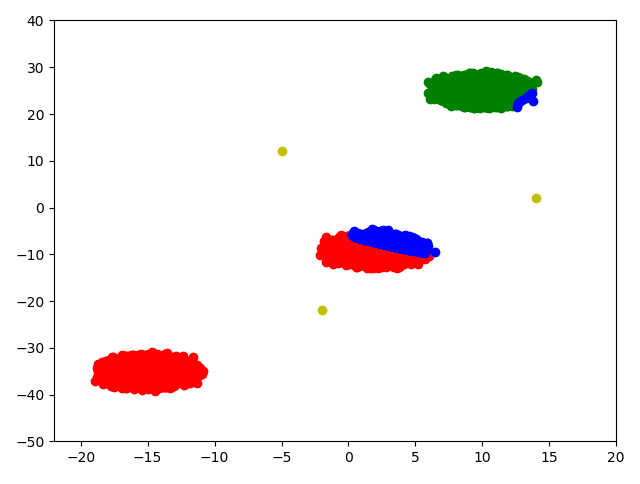
\includegraphics[width=0.6\textwidth]{../images/before_kmeans.png}\\
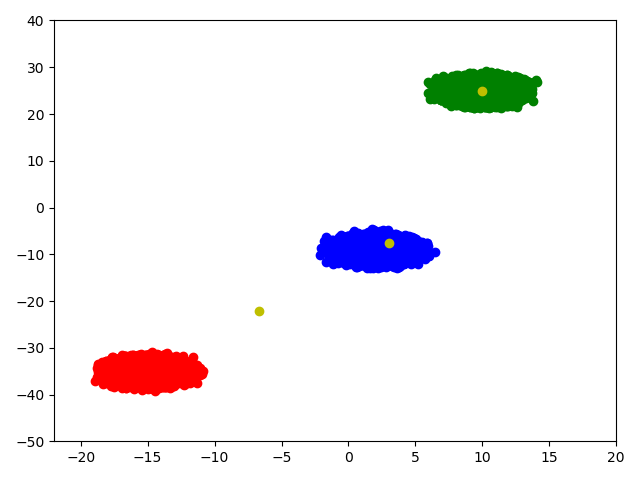
\includegraphics[width=0.6\textwidth]{../images/first_iteration.png}\\
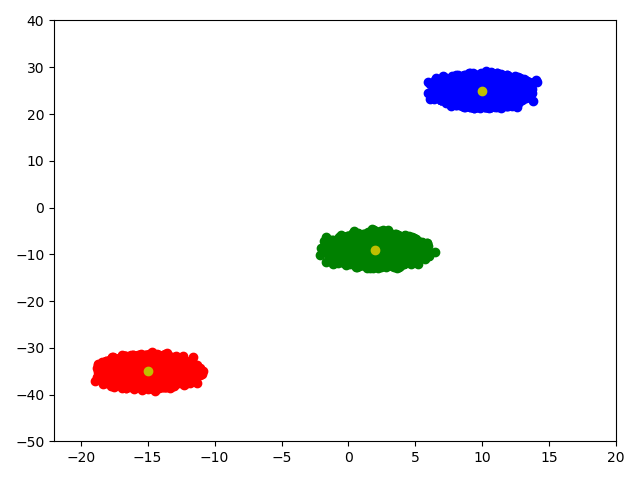
\includegraphics[width=0.6\textwidth]{../images/after_kmeans.png}\\
\end{center}



